% 请确保文件编码为utf-8,使用XeLaTex进行编译,或者通过overleaf进行编译

\documentclass[answers]{exam}  % 使用此行带有作答模块
% \documentclass{exam} % 使用此行只显示题目

\usepackage{xeCJK}
\usepackage{zhnumber}
\usepackage{graphicx}
\usepackage{hyperref}
\usepackage{amsmath}
\usepackage{booktabs}
\usepackage{enumerate}
\usepackage{amssymb}
\usepackage{listings}



\pagestyle{headandfoot}
\firstpageheadrule
\firstpageheader{南京大学}{高级机器学习}{习题集三}
\runningheader{南京大学}
{高级机器学习}
{习题集三}
\runningheadrule
\firstpagefooter{}{第\thepage\ 页(共\numpages 页)}{}
\runningfooter{}{第\thepage\ 页(共\numpages 页)}{}

% no box for solutions
% \unframedsolutions

\setlength\linefillheight{.5in}

% \renewcommand{\solutiontitle}{\noindent\textbf{答:}}
\renewcommand{\solutiontitle}{\noindent\textbf{解:}\par\noindent}

\renewcommand{\thequestion}{\zhnum{question}}
\renewcommand{\questionlabel}{\thequestion .}
\renewcommand{\thepartno}{\arabic{partno}}
\renewcommand{\partlabel}{\thepartno .}


\begin{document}
\Large

\begin{questions}
\question [30] \textbf{计算学习理论}

	本题探讨计算学习理论章节中VC 维的性质。
	
	\begin{parts}
		\part [10] 请在样本空间~$\mathcal{X} = [0,1]$~上构造一个有限假设空间~$\mathcal{H}$~使得~$\mbox{VC}(\mathcal{H}) = \left \lfloor \log_2(\left| \mathcal{H} \right| ) \right \rfloor $.
		
		\part [10] 定义轴平行四边形概念类~$\mathcal H = \{h_{(a_1, a_2, b_1, b_2)}(x, y): a_1\le a_2 \land b_1\le b_2\}$, 其中
		\[ h_{(a_1, a_2, b_1, b_2)}(x, y) = \begin{cases}
			1&\quad \text{ if } a_1\le x\le a_2 \land b_1\le y \le b_2 \\
			0 & \quad \text{otherwise}
		\end{cases}
		\]
		请证明~$\mathcal H$~的~VC~维为~4.
		
		\part [10] 请证明最近邻分类器的假设空间的~VC~维可以为无穷大.
		
	\end{parts}

	\begin{solution}
		\begin{parts}
			\part 令$\mathcal{H}$表示$[0,1]$上一些闭区间构成的集合\\
			$\{h_{[0.1,0.3]},h_{[0.3,0.5]},h_{[0.5,0.7]},h_{[0.1,0.8]}\}$,对$x\in\mathcal{X}$,有
			$$h_{[a,b]}(x)=
			\begin{cases}
				1\ \ x\in[a,b] \\
				0\ \ else 
			\end{cases}
		$$
			我们令$x_1=0.4,x_2=0.6$,不难发现$\mathcal{H}$中的假设将$\{x_1,x_2\}$打散,故$\mathcal{H}$的VC维至少是2\\
			~\\
			对于任意大小为3的示例集$\{x_3,x_4,x_5\}$,不妨设$x_3<x_4<x_5$,那么$\mathcal{H}$中没有一个假设可以实现如下对分结果$$\{(x_3,1),(x_4,0),(x_5,1)\}$$
			所以$\mathcal{H}$的VC维就是2,而$log_2(|\mathcal{H}|)=2$,所以构造出来的有限假设空间$\mathcal{H}$满足条件。

			\part 首先证明假设空间$\mathcal{H}$的VC维最小为4,\\
			令$(x_1,y_1)=(1.1,0),(x_2,y_2)=(0,1.1),$\\$(x_3,y_3)=(-1.1,0),(x_4,y_4)=(0,-1.1)$,
			存在假设(括号中数字代表分类结果)\\
			$\{h_{(0,1,0,1)}(0000),h_{(1,2,0,2)}(1000),h_{(0,1,0,2)}(0100),h_{(-2,0,0,1)}(0010),$\\
			$h_{(0,1,-2,0)}(0001),h_{(0,2,0,2)}(1100),h_{(-2,2,0,1)}(1010),h_{(0,2,-2,0)}(1001),$\\
			$h_{(-2,0,0,2)}(0110),h_{(0,1,-2,2)}(0101),h_{(-2,0,-2,0)}(0011),h_{(-2,2,0,2)}(1110),$\\
			$h_{(0,2,-2,2)}(1101),h_{(-2,2,-2,0)}(1011),h_{(-2,0,-2,2)}(0111),h_{(-2,2,-2,2)}(1111)\}$\\
			即如第三小问后的图片所示,可以作出一个矩形包含4个点中任意数目的点。\\
			接下来证明对任意大小为5的示例集$\{z_i=(x_i,y_i)\}_{i=1}^5$,不妨假设$x_5,y_5$都是五个点的坐标中第三大的,其中$z_1,z_2$在$z_5$上方,$z_3,z_4$在下方,此时$\{z_1,z_2\}$和$\{z_3,z_4\}$必然不可能在$z_5$的同侧(否则不满足$z_5$的横坐标也是第三大的要求),
			故假设$z_1$在$z_5$左侧,$z_3$在右侧\\
			那么不存在任何假设能实现对分结果$\{(z_1,1),(z_3,1),(z_5,0)\}$,故$\mathcal{H}$的VC维为4\\
			

			\part 对于最近邻分类器,它总是会将样本分类到与自己所属的类相同的类(因为样本到自身的距离最近),
			所以对于任意数量的样本,它的训练误差恒为0,所以其VC维可以为无穷大
		\end{parts}
	\end{solution}

	\begin{figure}[h]
		\centering
		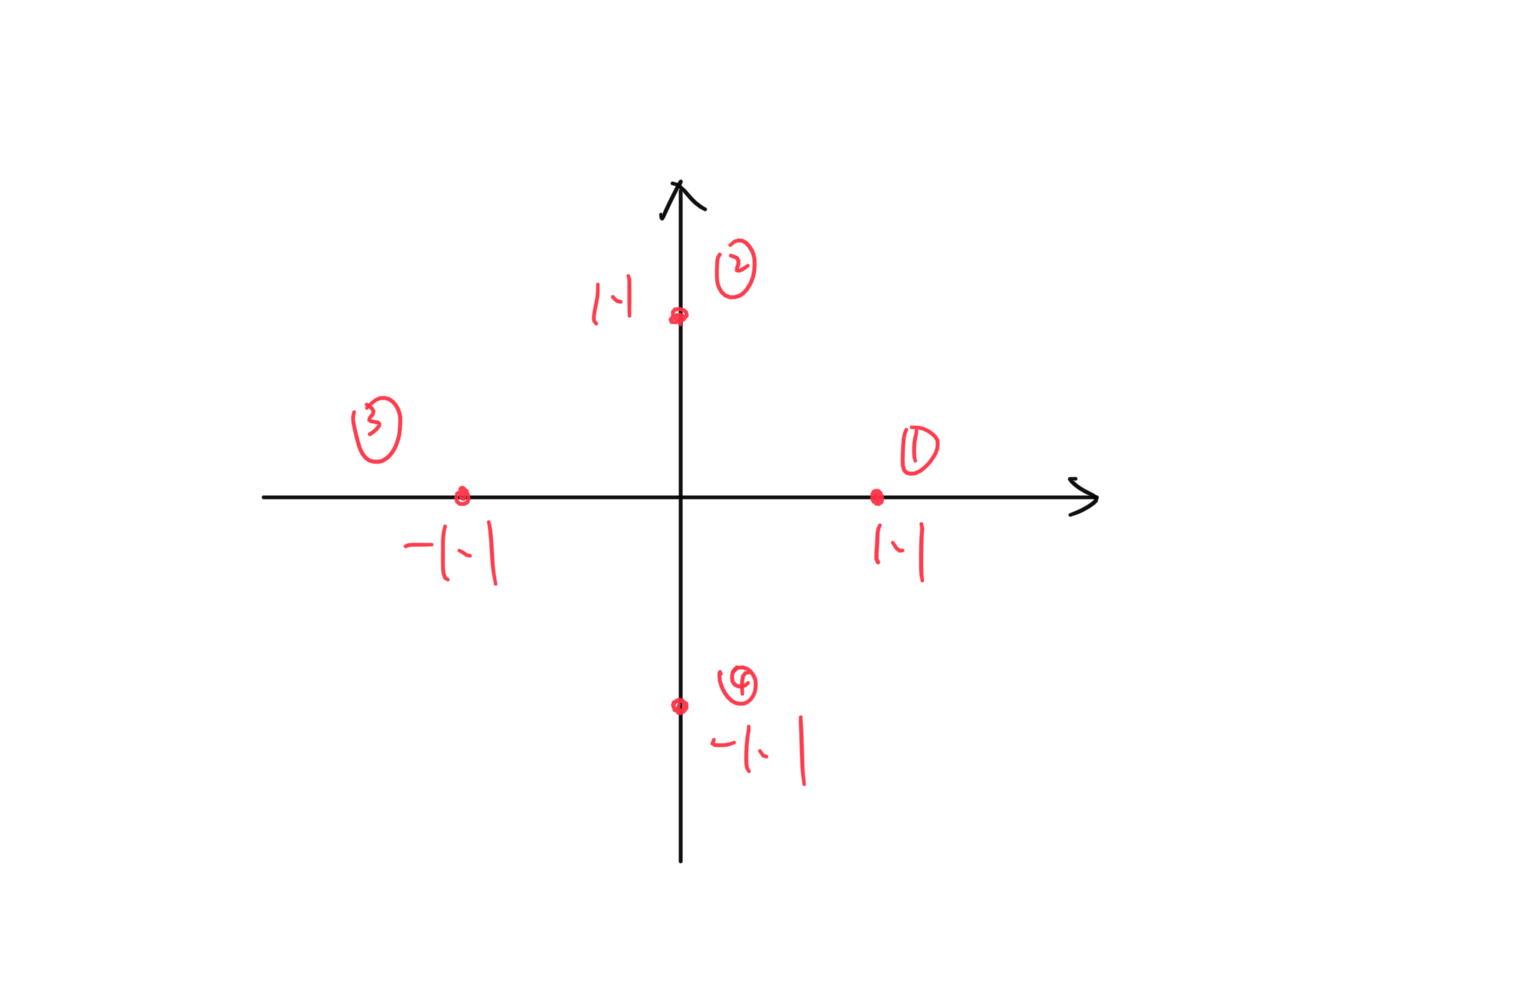
\includegraphics[width=0.7\linewidth,height=6cm]{p1-2.PNG}
		\caption{第一题第2问附图}
	\end{figure}
\newpage
\question [40] \textbf{编程题:特征工程和规则学习}

	\begin{figure}
		\centering
		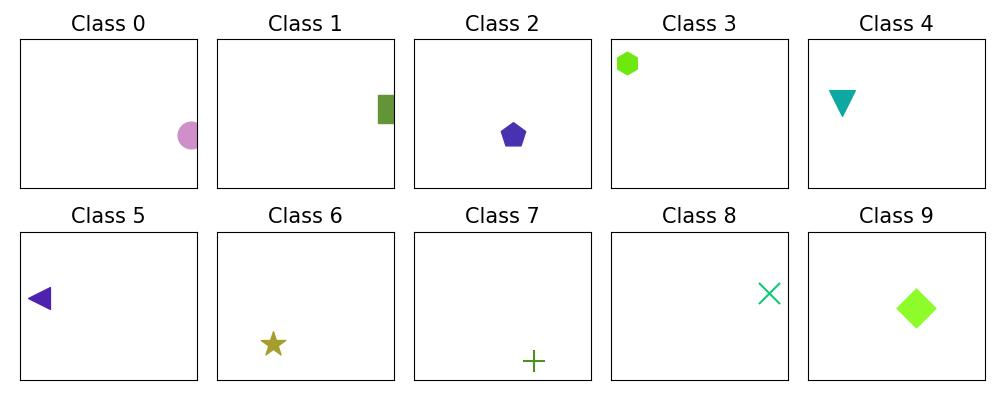
\includegraphics[width=0.7\linewidth]{problem2-code/demos/demo-0.jpg}
		\caption{图案分类问题示例图} \label{fig:q2-demo}
	\end{figure}

	本题涉及一个简单的图像识别问题,主要是对示例图~\ref{fig:q2-demo}中的10种图案进行识别,图案有不同大小、不同颜色,并且处在图像中不同位置,即不一定在中心位置,可能出现部分观测(某部分可能缺失,例如图中的Class 0)。分类依据主要是其形状,例如五角星、三角形、加号、正方形等等。本题代码文件夹在``problem2-code"目录下。\textbf{请在作答中贴出核心代码文件和结果,以方便批改。}
	
	\begin{parts}
		\part [10] 根据``generate\_samples.py"生成训练测试图片,其中n\_samples控制了训练测试样本中每个类别的数目,示例文件设置为200,那么训练测试集各有2000个样本。生成好图像之后,``load\_data.py"提供了读取图像数据的示例代码,``train\_p0.py"提供了使用对数几率回归(Logistic Regression)、决策树(Decision Tree)、随机森林(Random Forest)进行分类的示例代码。该代码还提供了可做PCA降维的选项。该代码没有提取任何特征,只是对图像缩放为32 * 32大小的彩色图像,然后使用所有像素点组成的向量进行分类。尝试运行该代码,将结果记录下来。此外,鼓励使用更多的分类器、更多的超参数设置、更多的数据进行训练,对比一下这些设置是否可以提升性能?例如:增加训练数据数量是否会提升性能?
		\part [10] 考虑到图像分类只和其形状有关,和其大小、位置、颜色无关,所以尝试将图像变为灰度图、定位目标的中心位置并进行裁剪等操作,然后再进行同样的训练。试着比较这种数据预处理带来的性能提升。提示:高阶的数据预处理还可以将灰度图变为轮廓图或者提取边缘信息等。
		\part [10] 上述虽然去除了一些和分类任务无关的信息(例如:颜色),但是其使用的特征依然是像素点信息。尝试手动提取高质量的特征,例如:图案中直线的数量、直线角度、直线之间的位置关系、图案的面积等等。试着以尽量少的特征获得更好的分类性能。提取的特征越少,性能越好,分数越高。
		\part [10] 在上一问中,使用决策树进行分类。本质上决策树就是一系列规则,尝试将决策树训练得到的模型使用文本或者图形将这一系列规则描述出来,观察是否符合预期(例如: 有一条水平和一条垂直线的是加号),从而更加深入地了解该模型。
	\end{parts}
	
	解\\
	1. 先依次运行$generate\_samples.py,load\_data.py,train\_p0.py$,本次得到的结果如图所示
	\begin{figure}[h]
		\centering
		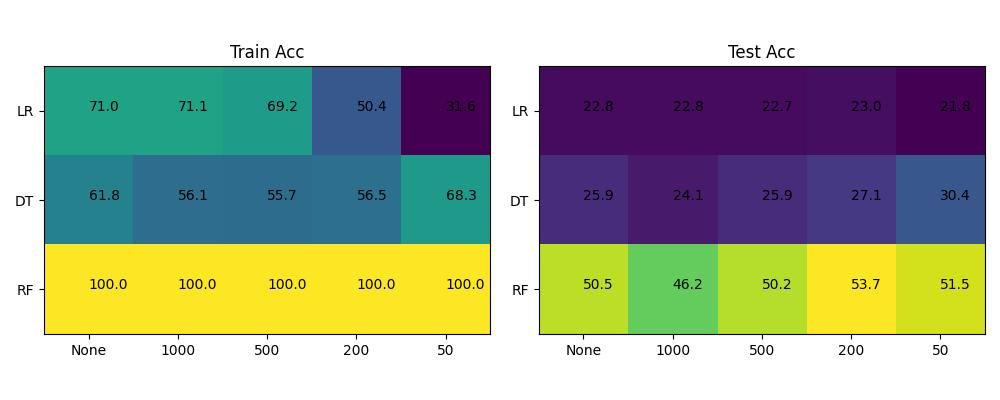
\includegraphics[width=15cm,height=8cm]{problem2-code/200-color.jpg}
		\caption{n-samples=200}
	\end{figure}

	接下来我加入了Lightgbm模型,并且分别在n-samples=100,200,300的条件下运行代码,得到了如下结果
\begin{lstlisting}[language={Python}]
     elif algo == "LGB":
         model = lgb.LGBMClassifier(
             max_depth=10
         )
\end{lstlisting}

	\newpage
	\begin{figure}[h]
		\centering
		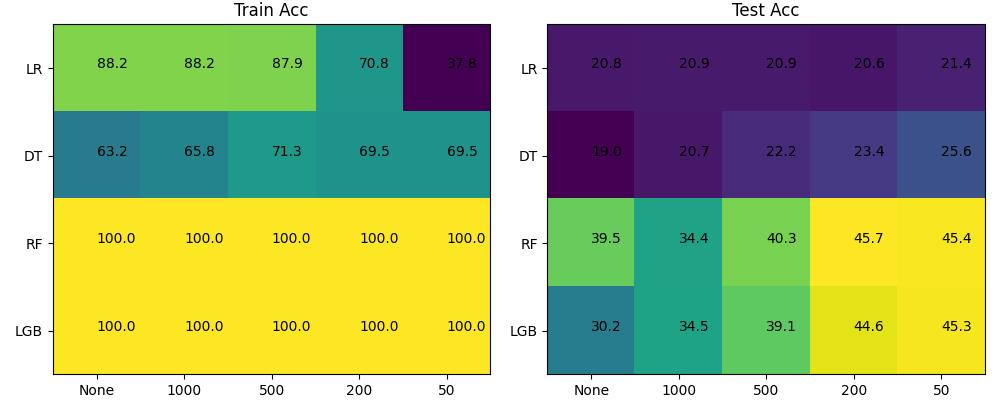
\includegraphics[width=15cm,height=7cm]{problem2-code/100-color(4models).jpg}
		\caption{n-samples=100(4models)}
	\end{figure}

	\begin{figure}[h]
		\centering
		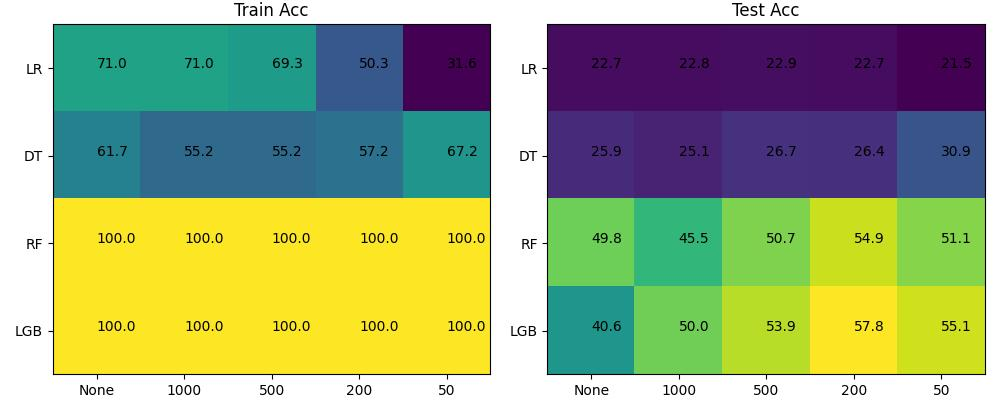
\includegraphics[width=15cm,height=7cm]{problem2-code/200-color(4models).jpg}
		\caption{n-samples=200(4models)}
	\end{figure}
	\newpage
	\begin{figure}[h]
		\centering
		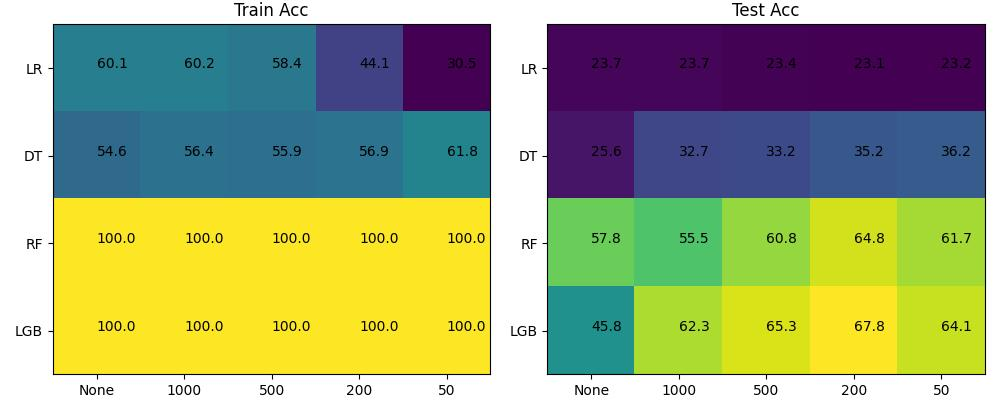
\includegraphics[width=15cm,height=8cm]{problem2-code/300-color(4models).jpg}
		\caption{n-samples=300(4models)}
	\end{figure}
	对比accuracy可见,增加样本数确实在一定程度上可以提高准确率(之所以没有加到400是因为此时训练耗时过长),
	而lightgbm的准确率相对而言也更好一些。\\
	~\\
	(2). 为节省训练耗时,后三问都只使用最初给定的三个模型并且n-samples设定为200\\
	首先,是将彩色图片统一变成灰度图,在$train\_p0.py$中定义了函数preprocess()并在其中添加如下代码:
	\begin{lstlisting}[language={Python}]
# 变成灰度图
for fname in os.listdir("figs/test"):
  img = Image.open(os.path.join("figs/test", fname))
  img = img.convert('L')
  img.save(os.path.join('figs_processed/test', fname))
for fname in os.listdir("figs/train"):
  img = Image.open(os.path.join("figs/train", fname))
  img = img.convert('L')
  img.save(os.path.join('figs_processed/train', fname))
	\end{lstlisting}
	此时,一个64*64的图像就对应着64*64的矩阵,每个值代表那个像素点的灰度值,并且越接近255就越接近白色,效果如图。\\
	\newpage
	\begin{figure}[h]
		\centering
		\includegraphics[width=8cm,height=8cm]{problem2-code/figs_processed/test/class0-0.jpg}
		\caption{test-class0-0灰度图}
	\end{figure}
	此时我们使用这些图片进行训练可以得到的结果如下:
	\begin{figure}[!h]
		\centering
		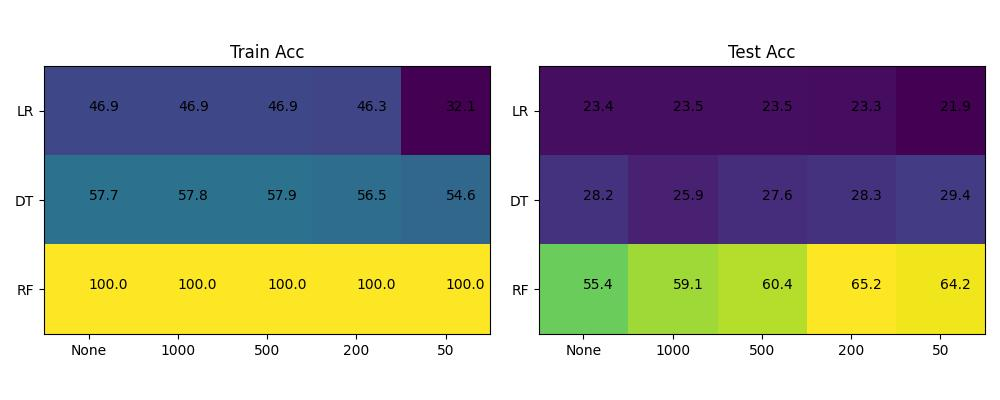
\includegraphics[width=15cm,height=8cm]{problem2-code/200_grey.jpg}
		\caption{只进行变灰}
	\end{figure}
	与(1)中的Figuer3对比可以发现,虽然略有提升,但效果也并不算很好,此时我们再对图片进行中心化:
\newpage
先是把每个图像都有的白色边框去除,依然是在preprocess()函数中添加代码,注:如下代码只能运行一次否则会导致图片出错
\begin{lstlisting}[language={Python}]
for fname in os.listdir("figs_processed/test"):
  img=Image.open(os.path.join("figs_processed/test",fname))
  img=img.crop((21, 16, 49, 44)) # 28*28
  img.save(os.path.join('figs_processed/test',fname))
for fname in os.listdir("figs_processed/train"):
  img=Image.open(os.path.join("figs_processed/train",fname))
  img=img.crop((21, 16, 49, 44))
  img.save(os.path.join('figs_processed/train',fname))
\end{lstlisting}
其中(21,16,49,44)是根据任意一个样本获取的内部正方形图片的坐标,其大小为28*28\\
~\\
接下来我们对得到的图片获取中心,具体思路如下:对于一幅图片,我们分别获取他不是全白的最上、下、左、右四个位置,
框出来的长方形就是大致的中心提取。接下来给出代码:
另外定义函数middle\_get(),它会在preprocess()中被调用,由于获取训练、测试集各个样本对应的四个位置的操作逻辑上完全一致,在此就只给出
获取测试集中样本最下一行有颜色的位置的行号的部分,其余的改一下对应变量名和路径名即可
\newpage
\begin{lstlisting}[language={Python}]
def middle_get():
  for fname in os.listdir("figs_processed/test"):
    img = Image.open(os.path.join("path", fname))
    mat = np.array(img)  
'''
path是figs_processed,版面不够长放不下了
mat是28*28,
灰度L=0.299R+0.587G+0.114B,255为白色
下面是四个坐标
'''
    L = 0
    R = 0
    U = 0
    D = 0
# 取图像最下一行
    for i in range(0, 28):
      flag = 0
      for j in range(0, 28):
  	    if mat[i, j] < 220:
  	      flag = 1
		  D = i
		  break
	    if flag:
	 	  break
\end{lstlisting}
类似的可以取到图像最上最左最右所对应的位置,然后使用img.crop()就可以获取到图像的主体部分。
在实践中的问题和解决如下:\\
一、图片的颜色不能直接使用<255进行判定,对于绝大多数图片,其主体部分的灰度值都较小,有些230,240灰度值
的部分仍然是无关信息。\\
二、部分图片的主体部分灰度值也较大,这会导致我们设定的判定条件下得到的坐标在用于裁剪时会出错,此时我们对坐标(L,D,R,U)进行判定,如果
不满足L<R、D<U那么对该图片就不进行裁剪以避免出错。\\
三、针对问题二,设定较高的灰度值上限并不可行,因为大部分图片如果依照高灰度值裁剪的话几乎不会发生变化,达不到提取图像中心的效果。
\newpage
\begin{figure}[h]
	\centering
	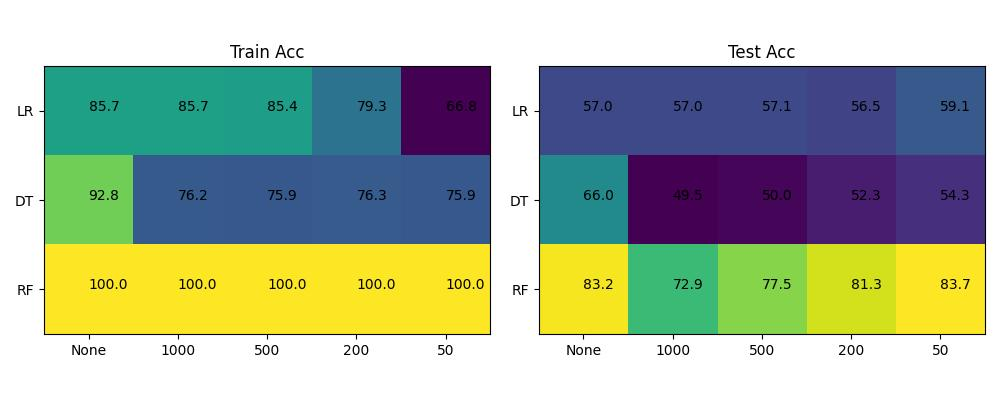
\includegraphics[width=15cm,height=7cm]{problem2-code/200-grey-cut.jpg}
	\caption{200\&grey\&cut}
\end{figure}
经过中心化裁剪后,相比于只进行变灰操作(Figure 8),很明显的看到accuracy有着较大提升\\
~\\
3. 本题中我手动提取了四项特征:图像的面积,图像中横线的数目,竖线的数目和线条的总数,代码如下(训练集和测试集方法完全一样,就不重复展示了)\\
大体思路是经过中心化裁剪的图片(除了class7和8),其图案部分的像素点大概率占图片的大部分,因此可以取图像矩阵的中位数的一定范围来对图案像素点进行判定。\\
而对于class7和8(加号和叉号),图像部分必然占少数,故用最小值来作为图案像素点的灰度值的估计。\\
获得了图案像素点的灰度值大致范围后,基于此我们可以计算图像的面积、横线数,竖线数等等。
\newpage
\begin{lstlisting}[language={Python}]
  for fname in os.listdir("figs_cut/test"):
	  img = Image.open(os.path.join("figs_cut/test", fname))
      mat = np.array(img)
      S = 0  # 面积
      line1 = 0  # 横线数
      line2 = 0  # 竖线数
      if fname.startswith("class") and fname.endswith(".jpg"):
          label1 = int(fname.split("-")[0][-1])
      if label1 == 7 or label1 == 8:
          maincolor = np.min(mat)
      else:
          maincolor = np.median(mat)
      for i in range(mat.shape[0]):
          for j in range(mat.shape[1]):
              if mat[i][j] > maincolor - 5 
	      and mat[i][j] < maincolor + 5:
                  S = S + 1  #
      for i in range(mat.shape[0]):
          for j in range(mat.shape[1]):
              if mat[i][j] > maincolor - 5 
		  and mat[i][j] < maincolor + 5 
		  and j < mat.shape[1] - 1:
                  if mat[i][j + 1] > maincolor - 5 
		  and mat[i][j + 1] < maincolor + 5:
                      line1 = line1 + 1
                      break

      for i in range(mat.shape[1]):
          for j in range(mat.shape[0]):
              if mat[j][i] > maincolor - 5 
		  and mat[j][i] < maincolor + 5 
		  and j < mat.shape[0] - 1:
                  if mat[j + 1][i] > maincolor - 5 
		  and mat[j][i] < maincolor + 5:
                      line2 = line2 + 1
                      break

      feature_test[count, 0] = S
      feature_test[count, 1] = line1
      feature_test[count, 2] = line2
      feature_test[count, 3] = line1 + line2
      label_test[count] = label1
      count = count + 1
		\end{lstlisting}
利用提取到的特征训练效果如图
\begin{figure}[h]
	\centering
	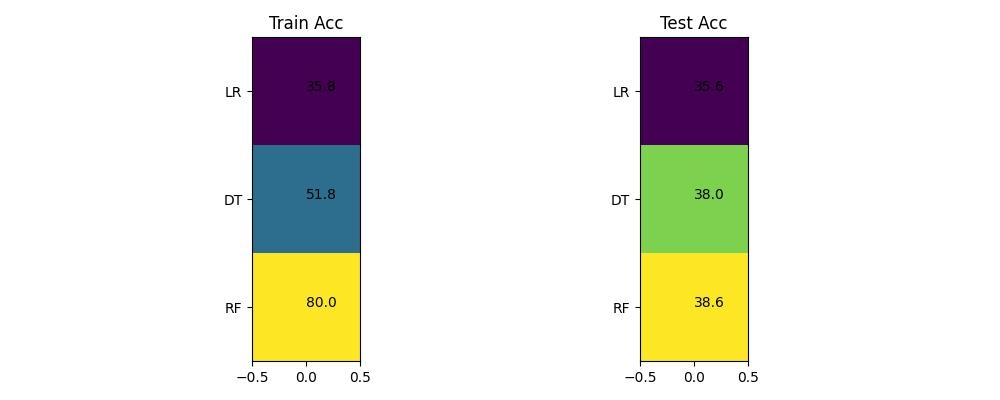
\includegraphics[width=0.7\linewidth]{problem2-code/feature-get.jpg}
	\caption{手动提取}
\end{figure}
效果并不是很好,个人认为原因在于手动提取的特征的质量相对较差,并且对于小部分图案颜色也接近白色的图片,采用范围来进行图案像素点
判定会导致整张图片都被判定成图案。\\
~\\
4. 决策树分类即为$Figure10$中的DT一行,依照提取的特征,可以概括规则如下:\\
\begin{align*}
&Rule1:\mbox{line1和line2(横线和竖线数)均=0,则为class8(叉号)}\\
&Rule2:\mbox{line1=1,line2=1,则为class7(加号)}\\
&Rule3:\mbox{面积S<某个值时,则为class7或8}
\end{align*}

\newpage
\question [30] \textbf{编程题:强化学习}
	\begin{figure}[h]
		\centering
		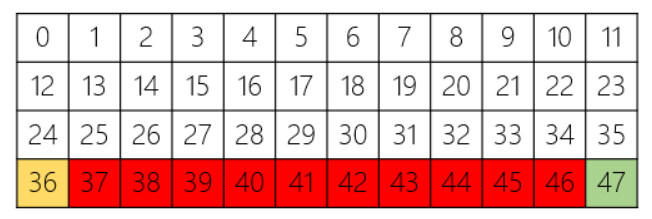
\includegraphics[width=0.7\linewidth]{problem3-code/env.PNG}
		\caption{悬崖行走问题示例图} \label{fig:q3-env}
	\end{figure}

	悬崖行走问题定义如下: 问题环境为如图~\ref{fig:q3-env}所示的4 * 12方格,智能体初始在36号位置,每次可上下左右移动一格,遇到墙则原地不动。每次移动获得-1奖励。37-46号位置为悬崖,若移动至悬崖,获得-100奖励并回到原点36号位置。47号位置为终点,运行至此为结束。总奖励为各步奖励之和。问题参数:$\epsilon=0.1,\alpha=0.5,\gamma=1$。\\
	请在悬崖行走问题中分别实现Sarsa算法与Q-learning算法,并分别输出运用两种算法训练得到的路径。本题代码文件夹在``problem3-code"目录下。问题环境可自己写,也可直接利用``cliff\_walking.py"文件中的Env类。\textbf{请在作答中贴出核心代码文件和结果,以方便批改。}
\newpage
	~\\
	~\\
		$\textbf{Sarsa}:$\\
		\begin{figure}[h]
			\centering
			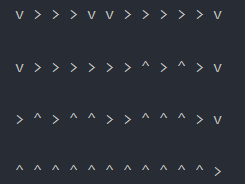
\includegraphics[width=0.7\linewidth,height=6cm]{problem3-code/sarsa.png}
			\caption{Sarsa路径图}
		\end{figure}
		~\\
		图中每个标记即为根据该点的$\max\limits_{a}q(s,a)$选出的最优动作,可以绘制出如下路线:	
		\begin{figure}[h]
			\centering
			\includegraphics[width=0.7\linewidth,height=8cm]{problem3-code/sarsa_way.png}
			\caption{Sarsa路径图}
		\end{figure}
		~\\
\newpage
		$\textbf{\mbox{核心代码}}$\\
		首先,将环境中未给出的到达终点的奖励补全\\
		\begin{lstlisting}[language={Python}]
#判定到达
def arrive(row, col):
	if row == 3 and col == 11:
		return 1
	else:
		return 0
#给出奖励(该部分代码在Env类中的transition函数下)
if (arrive(self.pos_row, self.pos_col)):
	return 100
\end{lstlisting} 
由于Sarsa算法和q-learning都要使用$\epsilon$-greedy策略,故提前写好方便调用:
\begin{lstlisting}[language={Python}]
def epsilon_greedy(policy, state, epsilon):
    # 探索
    if np.random.uniform(0, 1) < epsilon:
        return np.random.randint(0, 4)  # 随机选一个方向走

    # 利用
    else:
        return policy[state]#policy储存各个状态的最优行为
\end{lstlisting}
接下来我们完善Sarsa算法的流程:\\
首先对q表(设为48*4,每个状态对应4个行为)、策略、初状态、初状态的行为进行初始化:
\begin{lstlisting}[language={Python}]
    agent = Env(3, 0)#初状态
    state = agent.state
    action = np.random.randint(0, 4)#初始动作
    q_table = np.zeros([48, 4])#q表
    policy = []
    for i in range(0, 48):
        policy.append(np.random.randint(0, 4))  # 随机初始化策略
\end{lstlisting}
\newpage
接下来进行学习:
\begin{lstlisting}[language={Python}]
	t=100000#设定行动次数上限
    for i in range(0, t):
        r = agent.transition(action)#状态转移,得到回报
        next_state = agent.state#新状态
	#根据e-greedy选择新状态的行为
        next_action = epsilon_greedy(policy, next_state, e)
	#更新当前状态行为的q值
        q_table[state, action] += 
		alpha * (r + 
		gamma * q_table[next_state, next_action] 
		- q_table[state, action])
	#更新该状态的最优策略
        policy[state] = np.argmax(q_table[state, :])
	#更新当前状态和行为
        action = next_action
        state = next_state
\end{lstlisting}
最终输出相应的策略,将policy中的数字分别对应成上下左右打印出来即可,最终结果就如
开始的图片所示。
\newpage
		${\textbf{Q-learning}}:$\\
		\begin{figure}[h]
			\centering
			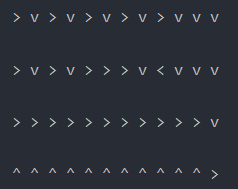
\includegraphics[width=0.7\linewidth,height=6cm]{problem3-code/q-learning.png}
			\caption{Sarsa路径图}
		\end{figure}
		~\\
		图中每个标记即为根据该点的$\max\limits_{a}q(s,a)$选出的最优动作,可以绘制出如下路线:	
		\begin{figure}[h]
			\centering
			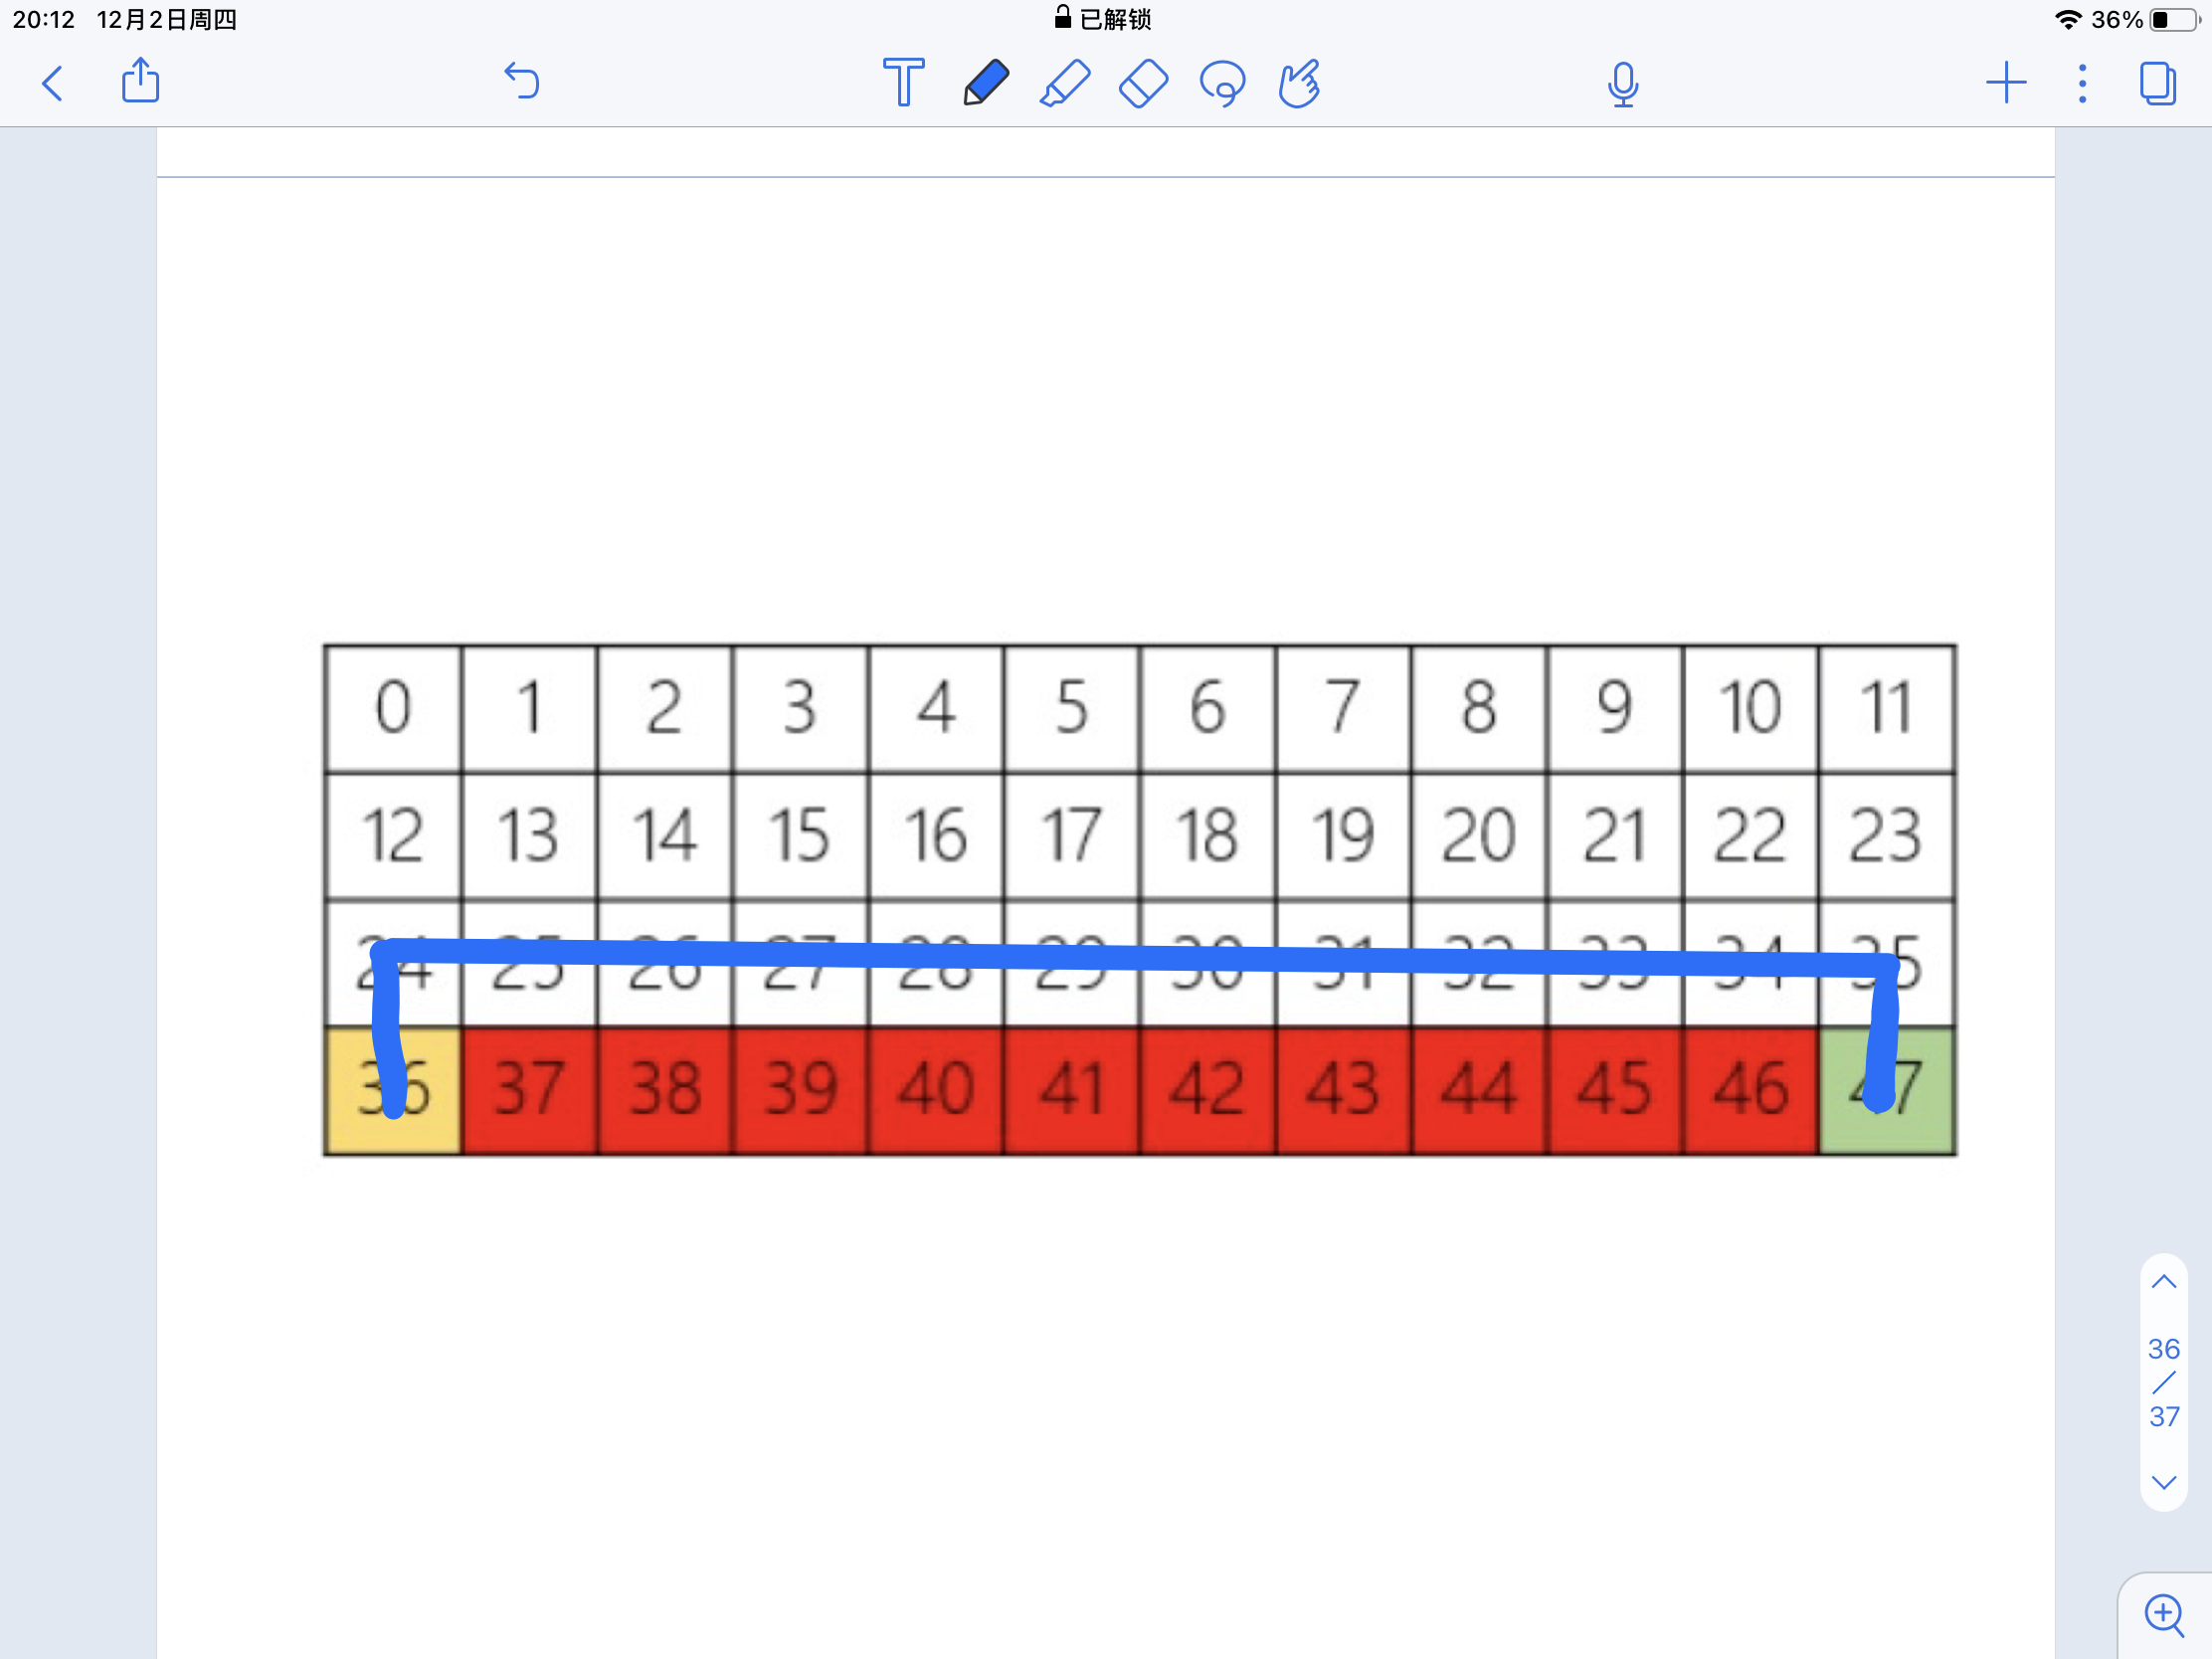
\includegraphics[width=0.7\linewidth,height=8cm]{problem3-code/q-learning_way.PNG}
			\caption{Sarsa路径图}
		\end{figure}
		~\\
		不难看出,Sarsa算法更偏向于走相对安全的路径,而Q-learning算法则是选择了全局最优的路径。\\
\newpage
		$\textbf{\mbox{核心代码}}$\\
		补全环境中的到达奖赏的代码已经放在Sarsa的代码中,此处就不再重新贴了。\\
		算法初始化与Sarsa有所不同,q-learning并没有随机化的选择初状态的动作,仅初始化了q表、策略、初状态,代码如下:
\begin{lstlisting}[language={Python}]
    policy = []
    for i in range(0, 48):
        policy.append(np.random.randint(0, 4))#随机初始化策略
    agent = Env(3, 0)  # 初始化状态
    state = agent.state
    q_table = np.zeros([48, 4])  # q值全部初始化为0
\end{lstlisting}
		接下来是q-learning过程代码:
\begin{lstlisting}[language={Python}]
    t=100000#最大行动次数
    for i in range(0, t):
	#使用e_greedy选择当前状态的行为
        action = epsilon_greedy(policy, agent.state, e)
	#进行转移并获得相应的回报
        r = agent.transition(action)
	#新状态
        next_state = agent.state
	#根据原始策略(即我们认为的最优策略)选择新状态的行为
        next_action = policy[next_state]
	#更新当前状态行为对的q值
        q_table[state, action] += alpha * (r + 
		gamma * q_table[next_state, next_action] 
		- q_table[state, action])
	#更新当前状态的策略
        policy[state] = np.argmax(q_table[state, :])
	#更新状态和行为
        action = next_action
        state = next_state
\end{lstlisting}
	最终根据q表得到策略,按照策略输出路径即可
\end{questions}


\end{document}